In \secref{prior_perturbations} we considered a multiplicative perturbations
of the form \eqref{phi_perturbation} with the $\norminf{\cdot}$ norm.  In
this section we consider other norms, illustrating that other choices
have problems with KL divergence.

First, we recall what we hope to get from our linear approximation.  We wish to
approximation $\etaopt(\phi)$ using the linear approximation $\etalin(\phi)$
evaluated at $\phiz$, hoping that the error $\norm{\etaopt(\phi) -
\etalin(\phi)}_2$ is small whenever the $\norm{\phi}$ is small (for some choice
of $\norm{\cdot}$).  A bare minimum for such a local approximation to work is
for $\phi \mapsto \etaopt(\phi)$ to be continuous, so that, for any
$\phi$,
%
\begin{align*}
%
\lim_{t \rightarrow 0} \norm{\etaopt(t \phi) - \etaopt}_2 = 0.
%
\end{align*}
%
By this reasoning, however, $\etaopt$ itself is a ``good'' approximation to
$\etaopt(\phi)$ when $\norm{\phi}$ is small---when $\phi$ is small, by
continuity we can simply say that nothing has changed and be reasonably correct.
From our linear approximation, we expect another order of accuracy, namely that
%
\begin{align*}
%
\lim_{t \rightarrow 0} \frac{\norm{\etaopt(t \phi) - \etalin(t\phi)}_2}{t} = 0.
%
\end{align*}
%
That is, we expect an extra order of accuracy from our linear approximation
in $\norm{\phi}$.

The preceding display is enough if we have a fixed $\phi$ in mind.  However, if
we want to search over a larger set of candidate $\phi$, we want the derivative
to provide a {\em uniformly good approximation} to $\etaopt(\phi)$ amonst some
set of $\phi$, say, all bounded $\phi: \norm{\phi} \le 1$.  One way of
formalizing the notion of ``uniformaly good approximation'' follows.

%%%%%%%%%%%%%%%%%%%%%%%%%%%%%%%%%%%%%%%%%%%%%%%%%%%%%%%%%%%%%%%%%%%%%%%%%%%
%%%%%%%%%%%%%%%%%%%%%%%%%%%%%%%%%%%%%%%%%%%%%%%%%%%%%%%%%%%%%%%%%%%%%%%%%%%
\begin{defn}\deflabel{diffable_classes}
    (\citep[Definition 4.5]{zeidler:2013:functional})
%
Let $B_1$ and $B_2$ denote Banach spaces, and let $\ball_1 \subseteq B_1$ define
an open neighborhood of $\phi_0 \in B_1$.  Fix a function $f: \ball_1
\mapsto B_2$.

The function $f$ is {\em directionally differentiable} (also known as a Gateaux
differentiable) if there exists a bounded linear functional $f^{\mathrm{lin}}:
B_1 \mapsto B_2$ such that
%
\begin{align*}
%
\textrm{For any }\phi: \norm{\phi - \phi_0} = 1\textrm{, }
\lim_{t \rightarrow 0}
    \frac{f(\phi) - f(\phi_0) -
          f^{\mathrm{lin}}(t (\phi - \phi_0) )
         }{t} \rightarrow 0.
%
\end{align*}
%

Similarly, the function $f$ is {\em boundedly differentiable} (also known as
Fr{\'echet} differentiable) at $\phi_0$ if
%
\begin{align*}
%
\lim_{t \rightarrow 0}
    \sup_{\phi: \norm{\phi - \phi_0} = 1}
    \frac{f(\phi) - f(\phi_0) -
          f^{\mathrm{lin}}(t (\phi - \phi_0))
         }{t} \rightarrow 0.
%
\end{align*}
%
\end{defn}
%%%%%%%%%%%%%%%%%%%%%%%%%%%%%%%%%%%%%%%%%%%%%%%%%%%%%%%%%%%%%%%%%%%%%%%%%%%

Note that we used the same notation $f^{\mathrm{lin}}$ for both derivatives in
\defref{diffable_classes}.  In fact, if a function is compactly differentiable
then the two derivatives must coincide \citep[Proposition
4.8]{zeidler:2013:functional}, which justifies our presumptuous notation.

The difference between bounded and directional differentiability is whether the
linear approximation holds uniformly in $\phi$.  It is possible for functions to
be directionally but not boundedly differentiable even in $\mathbb{R}^2$, as the
following example demonstrates.

%%%%%%%%%%%%%%%%%%%%%%%%%%%%%%%%%%%%%%%%%%%%%%%%%%%%%%%%%%%%%%%%%%%%%%%%%
%%%%%%%%%%%%%%%%%%%%%%%%%%%%%%%%%%%%%%%%%%%%%%%%%%%%%%%%%%%%%%%%%%%%%%%%%
\begin{ex}\exlabel{r2_pathological}
%
Consider $(x_1, x_2) \in \mathbb{R}^2$ and the polar coordinates $r :=
\sqrt{x_1^2 + x_2^2}$ and $\theta := \arctan(x_2 / x_1)$.  Let $\{\pi k: k \in
\mathbb{Z} \}$ denote integer multiples of $\pi$.  Define
%
\begin{align*}
%
f(r, \theta) := \begin{cases}
\frac{r / | \sin \theta |}{1 + r / | \sin \theta |}
    & \textrm{when } \theta \notin \{\pi k: k \in \mathbb{Z}\}
    \textrm{ and } r > 0 \\
0. & \textrm{when } \theta \in \{\pi k: k \in \mathbb{Z}
    \} \textrm{ or }r = 0
%
\end{cases}
%
\end{align*}
%
Then $f$ has a directional derivative in every direction, but is not Fr{\'e}chet
differentiable.
%
\begin{proof}
%
By ordinary calculus, for any $\theta$, $\fracat{\partial f(r, \theta)}{\partial
r}{r=0} = 0$, so the linear approximation to $f(r, \theta)$ at $r=0$ is
identically zero.  However, for any $r$, there exists a $\theta(r)$ such that
$r / |\sin(\theta(r))| = 1$.  For such a choice of $\theta(r)$, the error in
the linear approximation is $f(r, \theta(r)) - 0 = 1/2$, which does not go
to zero as $r \rightarrow 0$.
%
\end{proof}
%
\end{ex}
%%%%%%%%%%%%%%%%%%%%%%%%%%%%%%%%%%%%%%%%%%%%%%%%%%%%%%%%%%%%%%%%%%%%%%%%%
%
%%%%%%%%%%%%%%%%%%%%%%%%%%%%%%%%%%%%%%%%%%%%%%%%%%%%%%%%%%%%%%%%%%%%%%%%%
%%%%%%%%%%%%%%%%%%%%%%%%%%%%%%%%%%%%%%%%%%%%%%%%%%%%%%%%%%%%%%%%%%%%%%%%%
\begin{figure}[h!]

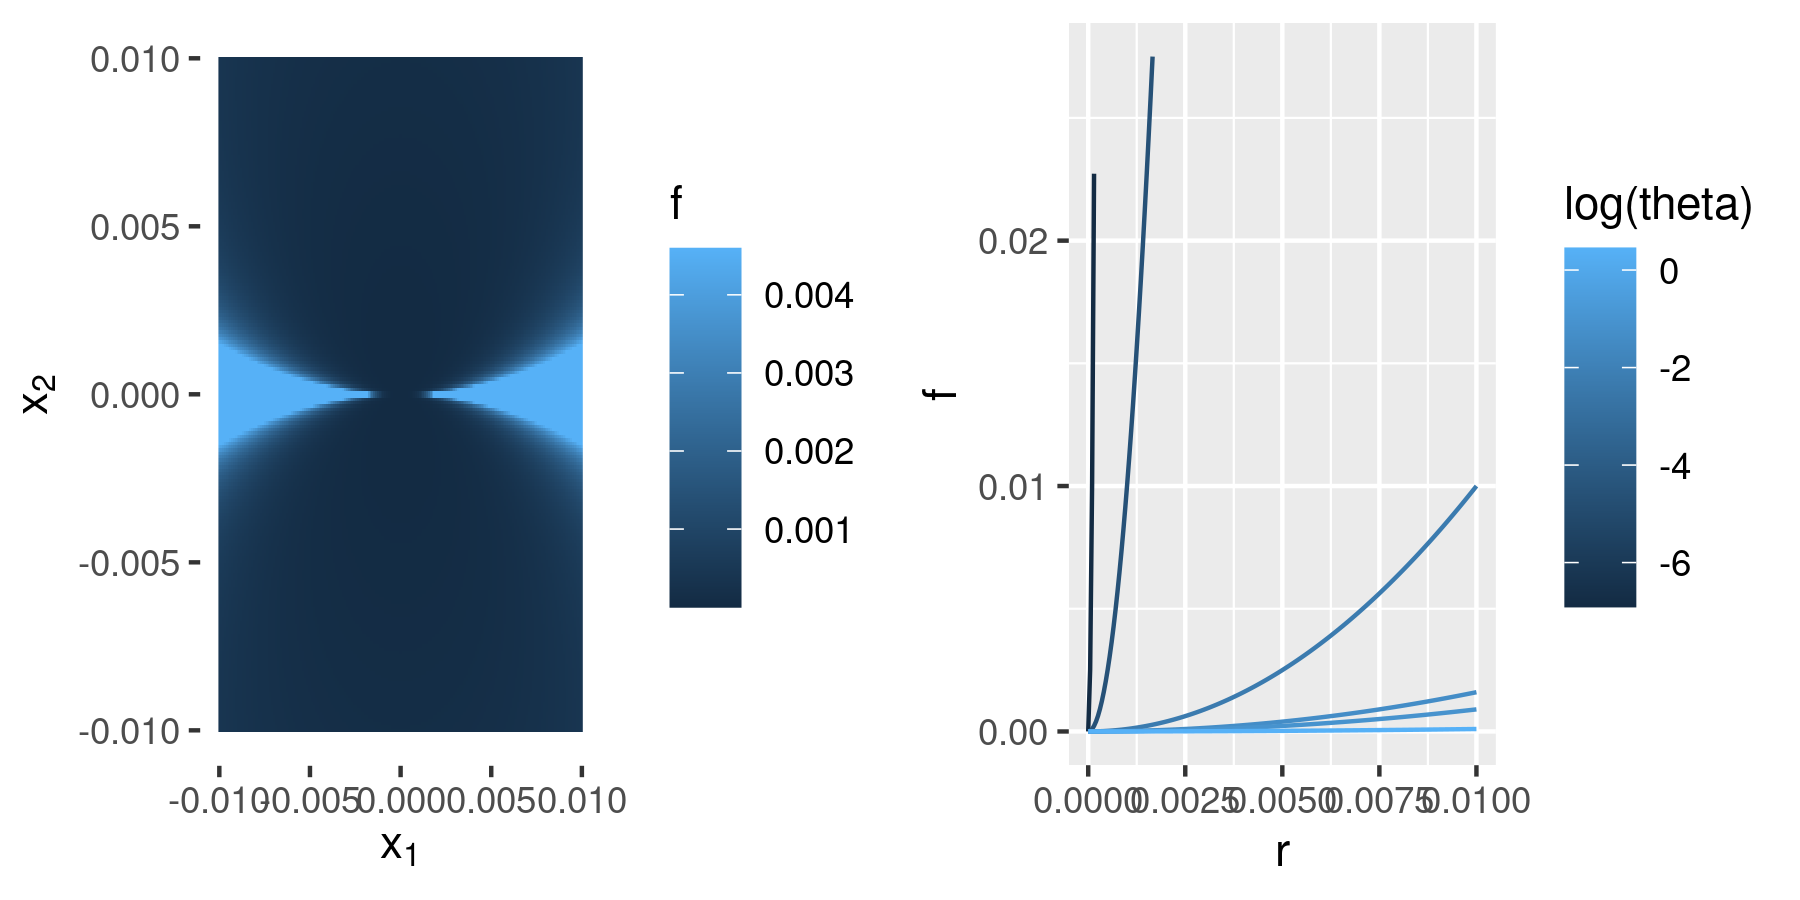
\includegraphics[width=0.980\linewidth,height=0.490\linewidth]{static_images/pathological_r2_example.png}
\caption{A plot of $f(x_1, x_2)$ from \exref{r2_pathological}.}\figlabel{r2_pathological}
\centering
\end{figure}
%%%%%%%%%%%%%%%%%%%%%%%%%%%%%%%%%%%%%%%%%%%%%%%%%%%%%%%%%%%%%%%%%%%%%%%%%



See \figref{r2_pathological} for a plot of \exref{r2_pathological}.


Another example is \citet[Example 1.9]{averbukh:1967:theory}.


-------------------

The above example is not the best.  What we want to say is that if a function is
Frechet differentiable then it is continuous.  (Zeidler Proposition 4.5 (d)). It
is possible to define discontinuous functions whose Gateaux derivatives exist.
And this is what we are worried about.  For this, a simpler R2 example will
suffice.  And we can use the function $\expect{\q(\theta)}{\log(1 +
\phi(\theta))}$ with the L2 norm as an example, which is perfect.
